% This must be in the first 5 lines to tell arXiv to use pdfLaTeX, which is strongly recommended.
\pdfoutput=1

\documentclass[11pt]{article}

% Change "final" to "review" if you want a submission with line numbers and anonymous authors
\usepackage[final]{acl}

% Standard package inclusions
\usepackage{times}
\usepackage{latexsym}
\usepackage[T1]{fontenc}
\usepackage[utf8]{inputenc}
\usepackage{microtype}
\usepackage{graphicx}
\usepackage{grffile}
\usepackage{amsmath}
\usepackage{booktabs}
\usepackage{hyperref}
\usepackage{url}

\title{Political Bias and Temporal Dynamics in Large Language Models}

\author{
  Ran Lu, Hasti Hosseinpour, Abderrahmane Moujar, Oloruntobi Olutola \\
  Université Paris-Saclay \\
  \texttt{\{first.last\}@universite-paris-saclay.fr}
}

\begin{document}
\maketitle

\begin{abstract}
Large Language Models (LLMs) are increasingly deployed as intermediaries for accessing, interpreting, and evaluating political information. Prior work has demonstrated that LLMs exhibit systematic political biases, reflected in ideological alignment, sentiment toward political actors, and framing choices. However, most existing studies treat political bias as a static property, evaluating models at a single point in time. This assumption overlooks the rapid evolution of LLMs, which undergo frequent updates to training data, safety mechanisms, and alignment procedures.

In this work, we investigate political bias as a temporal phenomenon, analyzing how political attitudes expressed by LLMs evolve across model generations. Focusing on longitudinal comparisons within model families, we examine how changes in safety data distributions and alignment interventions correspond to shifts in political stance and sentiment. Our study integrates Prediction Inconsistency (IC) and sentiment label distributions to provide a dynamic perspective on value alignment in large language models.
\end{abstract}

\section{Introduction}

Large Language Models (LLMs) have become central intermediaries in how individuals access, interpret, and evaluate political information. Their widespread use in tasks such as summarization, explanation, sentiment analysis, and question answering grants them substantial influence over contemporary digital public spheres. As these systems are increasingly embedded in search engines, social media platforms, and decision-support tools, their latent political orientations carry meaningful societal and political consequences.

A growing body of evidence suggests that LLMs are not ideologically neutral. Instead, political tendencies emerge from architectural decisions, training data composition, and post-training alignment strategies \citep{santurkar2023,buyl2026,hartmann2023,bang2024}. When models systematically favor or disfavor particular political ideologies, policies, or actors, they may function as implicit instruments of digital soft power.

Empirical research further shows that political bias in LLMs is not limited to isolated prompts but constitutes a structural property of model behavior. Studies have identified consistent ideological patterns across economic and social dimensions, as well as systematic sentiment differences toward political entities \citep{hartmann2023,bang2024}. Moreover, LLMs may exhibit bias amplification, whereby biases present in training data are reproduced or intensified in generated outputs \citep{zhu2024}.

Despite this progress, most prior work evaluates political bias under a static assumption, treating models as fixed artifacts. This perspective is increasingly inadequate given the rapid pace of LLM development. Model families such as Llama undergo substantial changes across generations, including modifications to training corpora, safety data distributions, and reinforcement learning-based alignment procedures \citep{touvron2023,dubey2024}.

\subsection{Research Questions and Contributions}

To address this gap, we study political bias through a temporal lens:
\begin{itemize}
  \item \textbf{RQ1:} How does political bias in LLM outputs change across successive model generations?
  \item \textbf{RQ2:} To what extent do safety alignment interventions correspond to shifts in political stance?
  \item \textbf{RQ3:} Are temporal changes in political bias uniform across ideological dimensions?
\end{itemize}

Our contributions are threefold: (1) we conceptualize political bias as a dynamic property; (2) we provide a longitudinal analysis across model generations using IC and label distributions; and (3) we link bias shifts to documented safety interventions.

\section{Related Work}

\subsection{Measuring Political Bias}
Early studies mapped LLM outputs onto ideological frameworks, demonstrating coherent political orientations. \citet{santurkar2023} argues models reflect aggregate training data opinions, while \citet{hartmann2023} situates ChatGPT along a left-libertarian axis. Target-oriented sentiment classification (TSC) further operationalizes bias by measuring sentiment toward specific actors \citep{wang2025,chen2024}.

\subsection{Temporal Dynamics}
Research shows LLMs exhibit temporal generalization failures, with biases drifting as contexts evolve \citep{zhu2024}. Between Llama 1, 2, and 3, Meta introduced changes to safety data and RLHF objectives \citep{touvron2023,dubey2024}. Comparative evaluations indicate newer models handle political nuance differently \citep{crum2024}.

\section{Methodology}

\subsection{Measuring Political Bias}
We adapt the framework proposed by \citet{elbouanani2025}, quantifying bias through Target-Oriented Sentiment Classification (TSC). 

\subsubsection{Data Selection}
We construct a set of 250 political figures across the ideological spectrum, ensuring diversity in gender, ethnicity, and geography. We select 60 news-style sentence templates (Positive, Negative, Neutral) that exclude role-specific references to maintain counterfactual consistency.

\subsubsection{Metrics}
We define Prediction Inconsistency (IC) as the instability of sentiment predictions when target entities are swapped. We derive the probability distribution for each label $l$:
\begin{equation}
P(l|s) = \frac{|\{e \in E : \text{pred}(s,e) = l\}|}{|E|}
\end{equation}
The Shannon entropy for a sentence is:
\begin{equation}
H(s) = -\sum_{l \in L} P(l|s) \log P(l|s)
\end{equation}
The global bias score is the average entropy: $\text{IC} = \frac{1}{m} \sum_{i=1}^{m} H(s_i)$.

\section{Results}

\subsection{ChatGPT}
IC is near zero for \texttt{gpt-3.5-turbo} but jumps to $\approx$0.67 for \texttt{gpt-4}, plateauing at $\approx$0.61 for later versions. While \texttt{gpt-3.5} assigned 100\% positive labels, \texttt{gpt-4} introduced a high share of UNKNOWN responses, reflecting increased hedging or refusal behavior. Figure~\ref{fig:chatgpt-ic} shows IC across ChatGPT versions; Figure~\ref{fig:chatgpt-ic-bar} gives a bar view; Figure~\ref{fig:chatgpt-labels} shows the label distribution.

\begin{figure}[t]
  \centering
  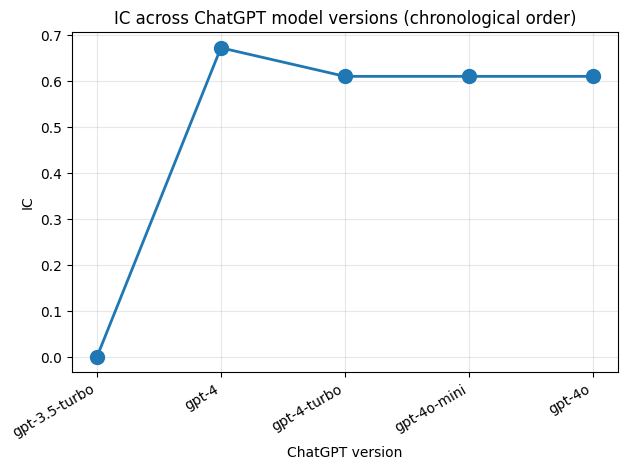
\includegraphics[width=\linewidth]{../figures/chatgpt_ic_chronological.png}
  \caption{Prediction Inconsistency (IC) across ChatGPT versions (chronological).}
  \label{fig:chatgpt-ic}
\end{figure}

\begin{figure}[t]
  \centering
  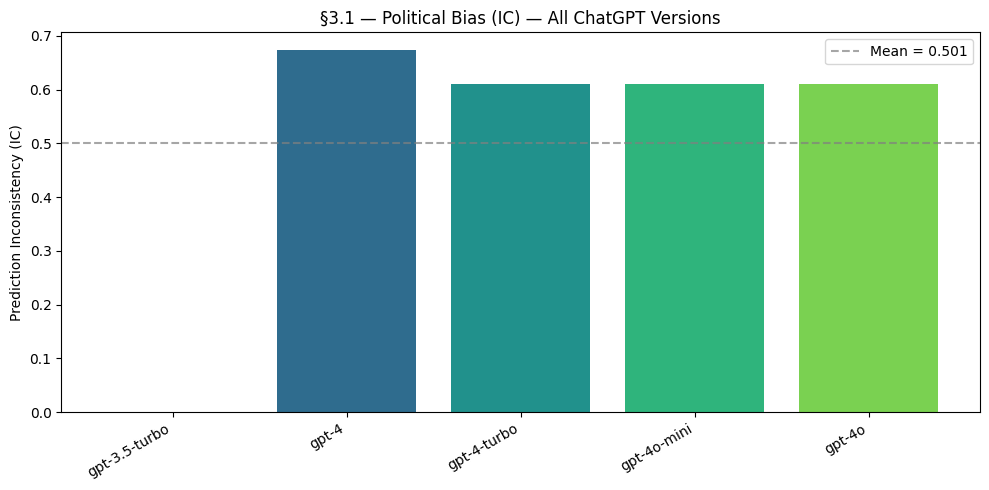
\includegraphics[width=\linewidth]{../figures/chatgpt_ic_bar.png}
  \caption{IC by ChatGPT model (bar chart).}
  \label{fig:chatgpt-ic-bar}
\end{figure}

\begin{figure}[t]
  \centering
  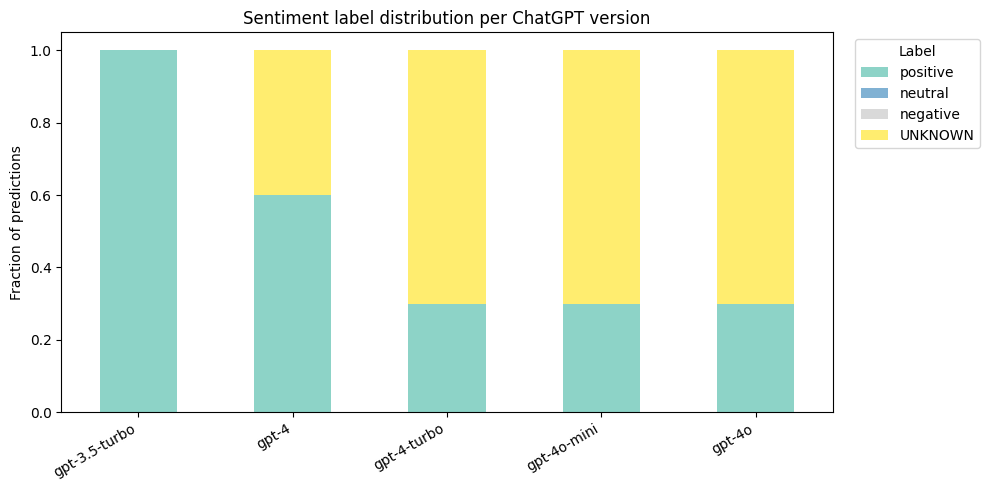
\includegraphics[width=\linewidth]{../figures/chatgpt_label_dist.png}
  \caption{Label distribution (positive, neutral, negative, UNKNOWN) for ChatGPT versions.}
  \label{fig:chatgpt-labels}
\end{figure}

\subsection{Llama}
We evaluate Llama~3.2 across model sizes and training stages (Figure~\ref{fig:llama-version}). IC decreases with model size (1B vs 3B) in the Base condition. Instruction tuning (Instruct) significantly reduces IC for the 1B and 11B models compared to their Base versions; the 3B model's IC remains relatively stable across alignment phases (Figure~\ref{fig:llama-pretrain-posttrain}). Figure~\ref{fig:llama-ic} shows IC for Base vs.\ Instruct variants; Figure~\ref{fig:llama-labels} shows the label distribution.

\begin{figure}[t]
  \centering
  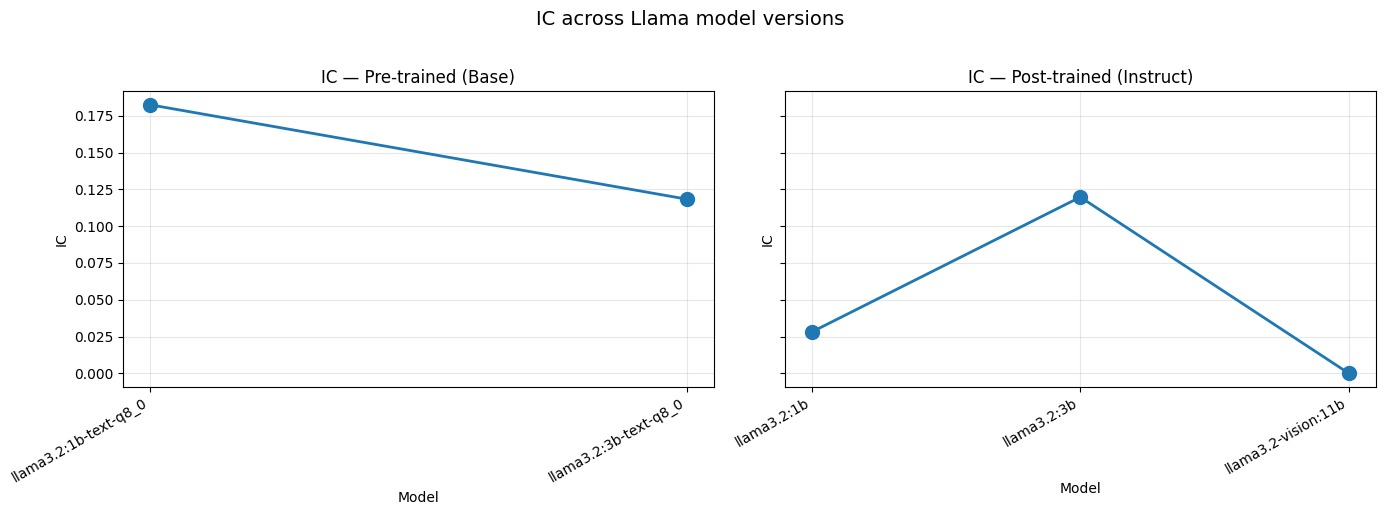
\includegraphics[width=\linewidth]{../figures/llama version.jpeg}
  \caption{Llama model versions evaluated (sizes and variants).}
  \label{fig:llama-version}
\end{figure}

\begin{figure}[t]
  \centering
  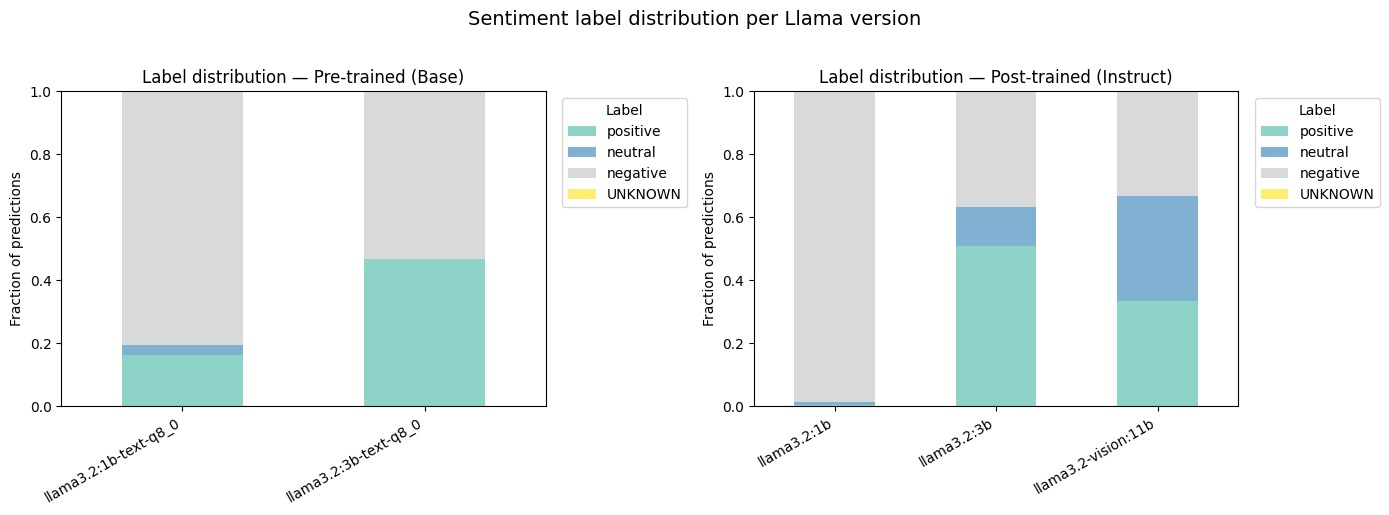
\includegraphics[width=\linewidth]{../figures/llama Pertraing post training.jpeg}
  \caption{Sentiment label distribution per Llama version: Pre-trained (Base) vs.\ Post-trained (Instruct).}
  \label{fig:llama-pretrain-posttrain}
\end{figure}

% \begin{figure}[t]
%   \centering
%   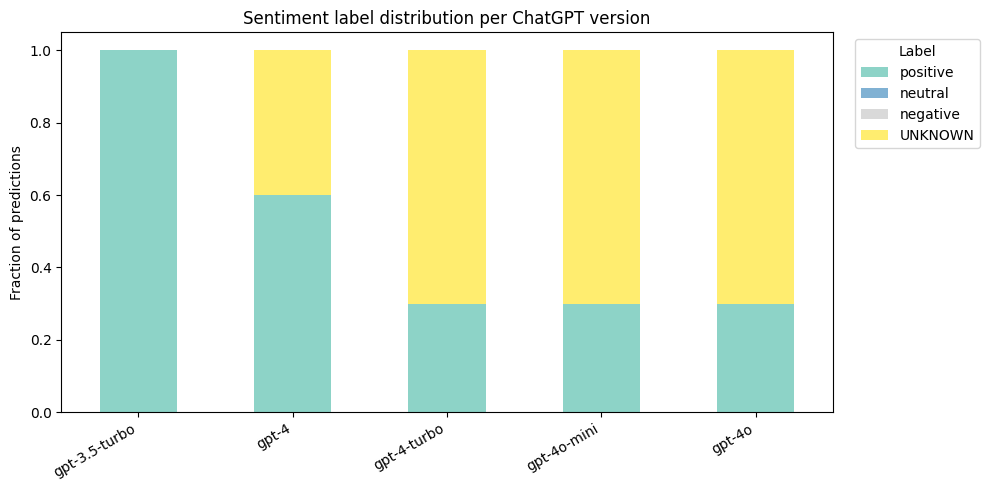
\includegraphics[width=\linewidth]{../figures/llama_ic_base_instruct.png}
%   \caption{Prediction Inconsistency (IC) for Llama~3.2 Base vs.\ Instruct variants.}
%   \label{fig:llama-ic}
% \end{figure}

% \begin{figure}[t]
%   \centering
%   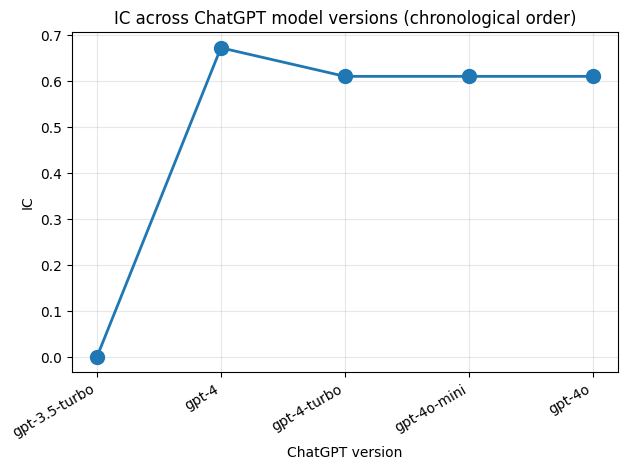
\includegraphics[width=\linewidth]{../figures/llama_label_dist.png}
%   \caption{Label distribution (positive, neutral, negative, UNKNOWN) for Llama models.}
%   \label{fig:llama-labels}
% \end{figure}

\subsection{Cross-family}
ChatGPT exhibits higher IC (0.61--0.67) than the Llama models we evaluated (0.005--0.178). ChatGPT outputs are dominated by positive and UNKNOWN; Llama models produce substantial negative and neutral shares.

\section{Discussion and Conclusion}
Political bias in LLMs is not static. For ChatGPT, bias (measured by IC) rose sharply with the transition to GPT-4. For Llama, bias mitigation via alignment is size-dependent. These findings underscore the necessity of longitudinal evaluations in AI ethics and value alignment research.


% Bibliography
\bibliographystyle{acl_natbib}
\bibliography{custom}

\end{document}